% ============================================================
%  Derivation: 2D Cartesian Coordinates (x, y)
%  Velocities: u (x-direction), v (y-direction)
%  Integration element: dx dy
% ============================================================

\section{2D Incompressible Flow in Cartesian Coordinates $(x,y)$}
\label{sec:cartesian}

\subsection{Governing Equations (Strong Form)}

For a 2D incompressible Newtonian fluid with constant properties and no body forces:

\textbf{Continuity:}
\begin{equation}
    \frac{\partial u}{\partial x} + \frac{\partial v}{\partial y} = 0
    \label{eq:cart_cont}
\end{equation}

\textbf{$x$-momentum:}
\begin{equation}
    \frac{\partial u}{\partial t}
    + \frac{\partial(u^2)}{\partial x}
    + \frac{\partial(uv)}{\partial y}
    = -\frac{1}{\rho}\frac{\partial p}{\partial x}
    + \frac{1}{\rho}\frac{\partial\tau_{xx}}{\partial x}
    + \frac{1}{\rho}\frac{\partial\tau_{xy}}{\partial y}
    \label{eq:cart_momx}
\end{equation}

\textbf{$y$-momentum:}
\begin{equation}
    \frac{\partial v}{\partial t}
    + \frac{\partial(uv)}{\partial x}
    + \frac{\partial(v^2)}{\partial y}
    = -\frac{1}{\rho}\frac{\partial p}{\partial y}
    + \frac{1}{\rho}\frac{\partial\tau_{xy}}{\partial x}
    + \frac{1}{\rho}\frac{\partial\tau_{yy}}{\partial y}
    \label{eq:cart_momy}
\end{equation}

where for a Newtonian fluid with constant viscosity $\mu = \rho\nu$:
\begin{align}
    \tau_{xx} &= 2\mu\frac{\partial u}{\partial x}
    \\
    \tau_{yy} &= 2\mu\frac{\partial v}{\partial y}
    \\
    \tau_{xy} &= \mu\!\left(\frac{\partial u}{\partial y}+\frac{\partial v}{\partial x}\right)
\end{align}

\textbf{Conservation vs.\ Convective Form:}
The equations above are written in \emph{conservation form}, where momentum fluxes appear explicitly as divergences (e.g.\ $\frac{\partial(u^2)}{\partial x}$ and $\frac{\partial(uv)}{\partial y}$). This differs from the \emph{convective form}, which expands the nonlinear terms using the product rule. To derive the convective form, expand the momentum flux divergences:
\begin{equation}
    \frac{\partial(u^2)}{\partial x} + \frac{\partial(uv)}{\partial y}
    = u\frac{\partial u}{\partial x} + u\frac{\partial u}{\partial x} + v\frac{\partial u}{\partial y} + u\frac{\partial v}{\partial y}
    = u\left(\frac{\partial u}{\partial x} + \frac{\partial v}{\partial y}\right) + u\frac{\partial u}{\partial x} + v\frac{\partial u}{\partial y}
\end{equation}
By the continuity equation $\frac{\partial u}{\partial x} + \frac{\partial v}{\partial y} = 0$, the first grouped term vanishes, leaving:
\begin{equation}
    \frac{\partial(u^2)}{\partial x} + \frac{\partial(uv)}{\partial y} = u\frac{\partial u}{\partial x} + v\frac{\partial u}{\partial y}
\end{equation}
This is the **convective form**. The conservation form is preferable for numerical schemes because it naturally encodes momentum balance at each cell: the divergence operators directly represent net flux in and out of the control volume, which the finite volume method integrates over CV boundaries. The convective form, while mathematically equivalent (under continuity), can miss discrete conservation properties in numerical discretization if not carefully constructed.

% ----------------------------------------------------------
\subsection{Staggered Grid Layout}
% ----------------------------------------------------------

A staggered (MAC) grid is used to avoid pressure--velocity decoupling.

\begin{figure}[H]
\centering
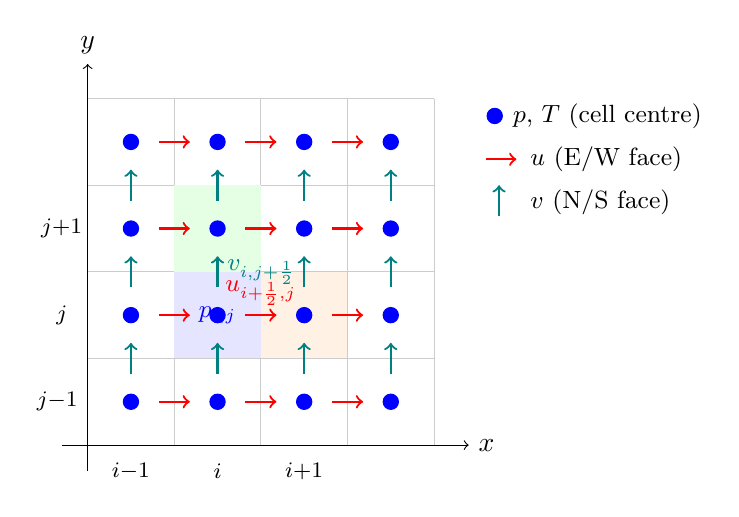
\begin{tikzpicture}[scale=1.1]
    % Grid lines
    \draw[gray!40, thin] (0,0) grid (4,4);

    % Highlight one control volume for p
    \fill[blue!10] (1,1) rectangle (2,2);
    \fill[green!10] (1,2) rectangle (2,3);
    \fill[orange!10] (2,1) rectangle (3,2);

    % Cell centers (pressure / scalar)
    \foreach \i in {0.5,1.5,2.5,3.5} {
        \foreach \j in {0.5,1.5,2.5,3.5} {
            \filldraw[blue] (\i,\j) circle (2.5pt);
        }
    }
    % u-faces (east/west faces)
    \foreach \i in {1,2,3} {
        \foreach \j in {0.5,1.5,2.5,3.5} {
            \draw[red,thick,->] (\i-0.18,\j) -- (\i+0.18,\j);
        }
    }
    % v-faces (north/south faces)
    \foreach \i in {0.5,1.5,2.5,3.5} {
        \foreach \j in {1,2,3} {
            \draw[teal,thick,->] (\i,\j-0.18) -- (\i,\j+0.18);
        }
    }

    % Labels for one cell
    \node[blue, font=\small] at (1.5,1.5) {$p_{i,j}$};
    \node[red,  font=\small, above] at (2,1.5) {$u_{i+\frac{1}{2},j}$};
    \node[teal, font=\small, right] at (1.5,2) {$v_{i,j+\frac{1}{2}}$};

    % Axes
    \draw[->] (-0.3,0) -- (4.4,0) node[right]{$x$};
    \draw[->] (0,-0.3) -- (0,4.4) node[above]{$y$};

    % Index labels
    \node[font=\footnotesize] at (0.5,-0.3) {$i{-}1$};
    \node[font=\footnotesize] at (1.5,-0.3) {$i$};
    \node[font=\footnotesize] at (2.5,-0.3) {$i{+}1$};
    \node[font=\footnotesize] at (-0.35,0.5) {$j{-}1$};
    \node[font=\footnotesize] at (-0.3,1.5) {$j$};
    \node[font=\footnotesize] at (-0.3,2.5) {$j{+}1$};

    % Legend
    \filldraw[blue] (4.7,3.8) circle (2.5pt);
    \node[font=\small, right] at (4.8,3.8) {$p$, $T$ (cell centre)};
    \draw[red,thick,->] (4.6,3.3) -- (4.95,3.3);
    \node[font=\small, right] at (5.0,3.3) {$u$ (E/W face)};
    \draw[teal,thick,->] (4.75,2.65) -- (4.75,3.0);
    \node[font=\small, right] at (5.0,2.8) {$v$ (N/S face)};
\end{tikzpicture}
\caption{Staggered Cartesian grid. Scalars ($p$, $T$) sit at cell centres (blue dots); $u$ is stored on east/west faces (red arrows); $v$ on north/south faces (teal arrows).}
\label{fig:cart_grid}
\end{figure}

% ----------------------------------------------------------
\subsection{Finite Volume Discretisation --- Integration over $\Delta x\,\Delta y$}
% ----------------------------------------------------------

Each equation is integrated over the appropriate control volume (CV) of area $\Delta x\,\Delta y$.

\subsubsection{Continuity Equation}

Integrating Eq.~\eqref{eq:cart_cont} over the scalar CV centred at $(i,j)$:
\begin{equation}
    \int_{\Delta y}\!\int_{\Delta x}
    \left(\frac{\partial u}{\partial x}+\frac{\partial v}{\partial y}\right)
    dx\,dy = 0
\end{equation}

Applying the divergence theorem (face fluxes):
\begin{equation}
    \frac{u_{i+\frac{1}{2},j} - u_{i-\frac{1}{2},j}}{\Delta x}
    + \frac{v_{i,j+\frac{1}{2}} - v_{i,j-\frac{1}{2}}}{\Delta y} = 0
    \label{eq:cart_disc_cont}
\end{equation}

\subsubsection{$x$-Momentum: CV at $(i+\tfrac{1}{2},\,j)$}

Integrating Eq.~\eqref{eq:cart_momx} over $[\,x_i,\,x_{i+1}\,]\times[\,y_{j-\frac{1}{2}},\,y_{j+\frac{1}{2}}\,]$:

\textbf{Temporal term:}
\begin{equation}
    \frac{\partial u_{i+\frac{1}{2},j}}{\partial t} \approx
    \frac{u_{i+\frac{1}{2},j}^{n+1} - u_{i+\frac{1}{2},j}^{n}}{\Delta t}
\end{equation}

\textbf{Convective terms} (central differencing):
\begin{align}
    u\frac{\partial u}{\partial x}\bigg|_{i+\frac{1}{2},j}
    &\approx u_{i+\frac{1}{2},j}\,
       \frac{u_{i+\frac{3}{2},j} - u_{i-\frac{1}{2},j}}{2\,\Delta x}
    \\[4pt]
    v\frac{\partial u}{\partial y}\bigg|_{i+\frac{1}{2},j}
    &\approx \bar{v}_{i+\frac{1}{2},j}\,
       \frac{u_{i+\frac{1}{2},j+1} - u_{i+\frac{1}{2},j-1}}{2\,\Delta y}
\end{align}
where $\bar{v}_{i+\frac{1}{2},j}
= \tfrac{1}{4}\!\left(v_{i,j+\frac{1}{2}}+v_{i+1,j+\frac{1}{2}}
                     +v_{i,j-\frac{1}{2}}+v_{i+1,j-\frac{1}{2}}\right)$
is the averaged $v$ at the $u$-face.

\textbf{Pressure gradient:}
\begin{equation}
    \frac{1}{\rho}\frac{\partial p}{\partial x}\bigg|_{i+\frac{1}{2},j}
    \approx \frac{1}{\rho}\frac{p_{i+1,j} - p_{i,j}}{\Delta x}
\end{equation}

\textbf{Viscous diffusion:}
\begin{equation}
    \nu\!\left(\frac{\partial^2 u}{\partial x^2}
              +\frac{\partial^2 u}{\partial y^2}\right)_{i+\frac{1}{2},j}
    \approx \nu\!\left(
      \frac{u_{i+\frac{3}{2},j}-2u_{i+\frac{1}{2},j}+u_{i-\frac{1}{2},j}}{\Delta x^2}
      +\frac{u_{i+\frac{1}{2},j+1}-2u_{i+\frac{1}{2},j}+u_{i+\frac{1}{2},j-1}}{\Delta y^2}
    \right)
\end{equation}

\subsubsection{$y$-Momentum: CV at $(i,\,j+\tfrac{1}{2})$}

By symmetry with the $x$-momentum equation:

\textbf{Convective terms:}
\begin{align}
    u\frac{\partial v}{\partial x}\bigg|_{i,j+\frac{1}{2}}
    &\approx \bar{u}_{i,j+\frac{1}{2}}\,
       \frac{v_{i+1,j+\frac{1}{2}} - v_{i-1,j+\frac{1}{2}}}{2\,\Delta x}
    \\[4pt]
    v\frac{\partial v}{\partial y}\bigg|_{i,j+\frac{1}{2}}
    &\approx v_{i,j+\frac{1}{2}}\,
       \frac{v_{i,j+\frac{3}{2}} - v_{i,j-\frac{1}{2}}}{2\,\Delta y}
\end{align}
where $\bar{u}_{i,j+\frac{1}{2}}
= \tfrac{1}{4}\!\left(u_{i+\frac{1}{2},j}+u_{i-\frac{1}{2},j}
                     +u_{i+\frac{1}{2},j+1}+u_{i-\frac{1}{2},j+1}\right)$.

% ----------------------------------------------------------
\subsection{Projection (Pressure-Correction) Method}
% ----------------------------------------------------------

\subsubsection{Step 1 --- Predictor (intermediate velocities $u^*$, $v^*$)}

Advance the momentum equations \emph{without} the pressure gradient:

\begin{equation}
\boxed{
u^{*}_{i+\frac{1}{2},j} = u^n_{i+\frac{1}{2},j}
+ \Delta t\left[
  -u^n_{i+\frac{1}{2},j}\frac{u^n_{i+\frac{3}{2},j}-u^n_{i-\frac{1}{2},j}}{2\Delta x}
  -\bar{v}^n_{i+\frac{1}{2},j}\frac{u^n_{i+\frac{1}{2},j+1}-u^n_{i+\frac{1}{2},j-1}}{2\Delta y}
  +\nu\!\left(
    \frac{u^n_{i+\frac{3}{2},j}-2u^n_{i+\frac{1}{2},j}+u^n_{i-\frac{1}{2},j}}{\Delta x^2}
    +\frac{u^n_{i+\frac{1}{2},j+1}-2u^n_{i+\frac{1}{2},j}+u^n_{i+\frac{1}{2},j-1}}{\Delta y^2}
  \right)
\right]
}
\label{eq:cart_pred_u}
\end{equation}

\begin{equation}
\boxed{
v^{*}_{i,j+\frac{1}{2}} = v^n_{i,j+\frac{1}{2}}
+ \Delta t\left[
  -\bar{u}^n_{i,j+\frac{1}{2}}\frac{v^n_{i+1,j+\frac{1}{2}}-v^n_{i-1,j+\frac{1}{2}}}{2\Delta x}
  -v^n_{i,j+\frac{1}{2}}\frac{v^n_{i,j+\frac{3}{2}}-v^n_{i,j-\frac{1}{2}}}{2\Delta y}
  +\nu\!\left(
    \frac{v^n_{i+1,j+\frac{1}{2}}-2v^n_{i,j+\frac{1}{2}}+v^n_{i-1,j+\frac{1}{2}}}{\Delta x^2}
    +\frac{v^n_{i,j+\frac{3}{2}}-2v^n_{i,j+\frac{1}{2}}+v^n_{i,j-\frac{1}{2}}}{\Delta y^2}
  \right)
\right]
}
\label{eq:cart_pred_v}
\end{equation}

\subsubsection{Step 2 --- Poisson Equation for Pressure Correction $p'$}

Enforcing $\nabla\cdot\mathbf{u}^{n+1}=0$ after the corrector step
$\mathbf{u}^{n+1}=\mathbf{u}^*-\Delta t\,\nabla p'/\rho$
yields the Poisson equation:

\begin{equation}
    \frac{\partial^2 p'}{\partial x^2}+\frac{\partial^2 p'}{\partial y^2}
    = \frac{\rho}{\Delta t}\left(
        \frac{\partial u^*}{\partial x}+\frac{\partial v^*}{\partial y}
      \right)
    \label{eq:cart_poisson}
\end{equation}

Discretised on the scalar CV at $(i,j)$:

\begin{equation}
\boxed{
\frac{p'_{i+1,j}-2p'_{i,j}+p'_{i-1,j}}{\Delta x^2}
+\frac{p'_{i,j+1}-2p'_{i,j}+p'_{i,j-1}}{\Delta y^2}
= \frac{\rho}{\Delta t}\left(
  \frac{u^*_{i+\frac{1}{2},j}-u^*_{i-\frac{1}{2},j}}{\Delta x}
  +\frac{v^*_{i,j+\frac{1}{2}}-v^*_{i,j-\frac{1}{2}}}{\Delta y}
\right)
}
\label{eq:cart_disc_poisson}
\end{equation}

This linear system $\mathbf{A}\,\mathbf{p}'=\mathbf{b}$ is solved at every time step (see Section~\ref{sec:cart_poisson_solver}).

\subsubsection{Step 3 --- Velocity Correction}

\begin{equation}
\boxed{
    u^{n+1}_{i+\frac{1}{2},j} = u^*_{i+\frac{1}{2},j}
    - \frac{\Delta t}{\rho}\,\frac{p'_{i+1,j}-p'_{i,j}}{\Delta x}
}
\label{eq:cart_corr_u}
\end{equation}

\begin{equation}
\boxed{
    v^{n+1}_{i,j+\frac{1}{2}} = v^*_{i,j+\frac{1}{2}}
    - \frac{\Delta t}{\rho}\,\frac{p'_{i,j+1}-p'_{i,j}}{\Delta y}
}
\label{eq:cart_corr_v}
\end{equation}

\subsubsection{Step 4 --- Pressure Update}

\begin{equation}
\boxed{
    p^{n+1}_{i,j} = p^{n}_{i,j} + \zeta\,p'_{i,j}
}
\label{eq:cart_pupdate}
\end{equation}

where $\zeta \in (0,1]$ is an under-relaxation factor (commonly $\zeta = 0.5$).

% ----------------------------------------------------------
\subsection{Poisson Solver Procedure}
\label{sec:cart_poisson_solver}
% ----------------------------------------------------------

Equation~\eqref{eq:cart_disc_poisson} can be rearranged to isolate $p'_{i,j}$:

\begin{equation}
    p'_{i,j} = \frac{1}{2\!\left(\dfrac{1}{\Delta x^2}+\dfrac{1}{\Delta y^2}\right)}
    \left[
        \frac{p'_{i+1,j}+p'_{i-1,j}}{\Delta x^2}
       +\frac{p'_{i,j+1}+p'_{i,j-1}}{\Delta y^2}
       - b_{i,j}
    \right]
    \label{eq:cart_gs}
\end{equation}

where
$b_{i,j} = \dfrac{\rho}{\Delta t}
\!\left(\dfrac{u^*_{i+\frac{1}{2},j}-u^*_{i-\frac{1}{2},j}}{\Delta x}
        +\dfrac{v^*_{i,j+\frac{1}{2}}-v^*_{i,j-\frac{1}{2}}}{\Delta y}\right)$.

\textbf{Iterative procedure (Gauss--Seidel or SOR):}
\begin{enumerate}
    \item Initialise $p'_{i,j}=0$ everywhere.
    \item Apply boundary conditions for $p'$ (Neumann $\partial p'/\partial n = 0$ at walls; $p'=0$ at outflow).
    \item Sweep all interior cells using Eq.~\eqref{eq:cart_gs}: \\
          SOR version: $p'^{\,\text{new}}_{i,j} = p'^{\,\text{old}}_{i,j} + \omega\!\left(p'^{\,\text{GS}}_{i,j}-p'^{\,\text{old}}_{i,j}\right)$, with $1 < \omega < 2$.
    \item Check convergence: $\max_{i,j}|p'^{\,\text{new}}_{i,j}-p'^{\,\text{old}}_{i,j}| < \varepsilon$.
    \item Repeat from step 2 until converged.
\end{enumerate}

\textbf{Alternatively --- Direct solver (LU / sparse):}
Assemble the $(N_x N_y)\times(N_x N_y)$ sparse matrix $\mathbf{A}$ from Eq.~\eqref{eq:cart_disc_poisson} and solve $\mathbf{A}\mathbf{p}'=\mathbf{b}$ once per time step using \texttt{scipy.sparse.linalg.spsolve} (or similar).

% ----------------------------------------------------------
\subsection{Ghost Cells and Boundary Conditions}
% ----------------------------------------------------------

Ghost (halo) cells are fictitious cells added one layer outside the physical boundary.  They allow interior-stencil formulas to be applied uniformly up to the boundary without special-casing.

\begin{figure}[H]
\centering
\begin{tikzpicture}[scale=1.0]
    % Physical domain (3x3 interior)
    \fill[blue!8] (1,0) rectangle (4,3);
    % Ghost cells top
    \fill[red!15] (1,3) rectangle (4,4);
    % Ghost cells bottom
    \fill[red!15] (1,-1) rectangle (4,0);
    % Ghost cells left
    \fill[red!15] (0,0) rectangle (1,3);
    % Ghost cells right
    \fill[red!15] (4,0) rectangle (5,3);
    % Ghost corners
    \fill[red!8] (0,-1) rectangle (1,0);
    \fill[red!8] (4,-1) rectangle (5,0);
    \fill[red!8] (0,3) rectangle (1,4);
    \fill[red!8] (4,3) rectangle (5,4);

    % Grid lines
    \draw[gray!60] (0,-1) grid (5,4);
    % Bold boundary
    \draw[black, very thick] (1,0) rectangle (4,3);

    % Labels
    \node[font=\small, blue] at (2.5,1.5) {Interior};
    \node[font=\small, red!70!black] at (2.5,3.5) {Ghost (top)};
    \node[font=\small, red!70!black] at (2.5,-0.5) {Ghost (bottom)};
    \node[font=\small, red!70!black, rotate=90] at (0.5,1.5) {Ghost};
    \node[font=\small, red!70!black, rotate=90] at (4.5,1.5) {Ghost};

    % BC annotation: no-slip wall at top
    \draw[<->, orange, thick] (5.3,3) -- (5.3,4);
    \node[orange, font=\small, right] at (5.4,3.5) {Ghost layer};
    \node[font=\footnotesize, right] at (5.4,2.8) {No-slip: $u_\text{ghost}=-u_\text{interior}$};
    \node[font=\footnotesize, right] at (5.4,2.4) {so that $u_\text{wall}=\tfrac{1}{2}(u_\text{i}+u_\text{g})=0$};

    % Axes
    \draw[->] (-0.2,-1.3) -- (5.2,-1.3) node[right]{$x$};
    \draw[->] (-0.5,-1.2) -- (-0.5,4.3) node[above]{$y$};
\end{tikzpicture}
\caption{Ghost cell (halo) layout for a 2D Cartesian domain. Red cells are ghost cells; blue cells are physical interior cells. The bold rectangle marks the physical boundary.}
\label{fig:cart_ghost}
\end{figure}

\textbf{How to set ghost cell values:}

\begin{center}
\begin{tabular}{llll}
\toprule
Boundary & Condition & Variable & Ghost cell value \\
\midrule
No-slip wall  & $u_w=0$, $v_w=0$  & $u$  & $u_\text{ghost} = -u_\text{interior}$ \\
              &                   & $v$  & $v_\text{ghost} = -v_\text{interior}$ \\
              & $\partial p/\partial n=0$ & $p$ & $p_\text{ghost} = p_\text{interior}$ \\
\midrule
Symmetry (e.g.\ centreline) & $\partial u/\partial y=0$ & $u$ & $u_\text{ghost} = u_\text{interior}$ \\
                             & $v=0$ & $v$ & $v_\text{ghost} = -v_\text{interior}$ \\
\midrule
Inlet & $u=U_\text{in}$, $v=0$ & $u$ & $u_\text{ghost} = 2U_\text{in}-u_\text{interior}$ \\
\midrule
Outlet (zero-gradient) & $\partial(\cdot)/\partial x=0$ & any & $\phi_\text{ghost}=\phi_\text{interior}$ \\
\bottomrule
\end{tabular}
\end{center}

The ghost cell value is computed \emph{before} each Runge--Kutta or Adams--Bashforth stage so that boundary conditions are enforced at the correct sub-step.
